\documentclass[conference]{IEEEtran}
\IEEEoverridecommandlockouts

\usepackage{cite}
\usepackage{amsmath,amssymb}
\usepackage{graphicx}
\usepackage{booktabs}
\usepackage{array}
\usepackage{microtype}
\usepackage[hidelinks]{hyperref}

\graphicspath{{images/}}

\begin{document}

\title{Policy-Guided Real-Time Mentoring for Introductory Programming Feedback}

\author{
    \IEEEauthorblockN{Alimzhan Koshikov}
    \IEEEauthorblockA{
        School of Software Engineering\\
        Astana IT University\\
        Astana, Kazakhstan\\
        225148@astanait.edu.kz\\
        \href{https://orcid.org/0009-0003-3234-6487}{0009-0003-3234-6487}
    }
    \and
    \IEEEauthorblockN{Tutkyshbayeva Shyryn}
    \IEEEauthorblockA{
        School of Software Engineering\\
        Astana IT University\\
        Astana, Kazakhstan\\
        sh.tutkyshbayeva@astanait.edu.kz\\
        \href{https://orcid.org/0000-0002-1419-2571}{0000-0002-1419-2571}
    }
}

\maketitle

\begin{abstract}
Introductory programming students often receive compiler messages and failed tests quickly, but they do not always receive feedback that is timely, limited, and safe for learning. A beginner who is stuck on a loop boundary or a wrong condition may need a small nudge, not a complete generated answer. This paper presents SocratesAI, a real-time virtual mentor for CS1 programming that separates feedback action selection from feedback wording. The system analyzes code states, keeps a compact session state, and applies a pedagogical policy before producing any student-facing message. The policy selects one of four actions: code-region highlight, conceptual hint, guiding question, or no feedback. A language model is used only after this action is selected, so it realizes a bounded intervention instead of deciding the tutoring strategy by itself. The prototype was evaluated through a real-HTTP PostgreSQL replay, a concurrent stress test, a 12-problem rubric benchmark, a 381,003-row weak-label policy dataset, and model comparison with ablations. In the latest valid ML+Gemini benchmark, SocratesAI processed 360 problem-suite events across 12 tasks with 0 runtime errors, 95.83\% agreement with target feedback actions, 95.80\% macro F1, mean latency of 1079.21 ms, and P95 latency of 2072 ms. The ablation study showed that removing analyzer-derived features reduced macro F1 from 1.0000 to 0.8813 on the expanded dataset. The results support technical feasibility and action-selection validity, while learning-gain claims still require a classroom study.
\end{abstract}

\begin{IEEEkeywords}
CS1, programming education, real-time feedback, virtual mentor, student modeling, policy learning, LLM-assisted education
\end{IEEEkeywords}

\section{Introduction}

Introductory programming is difficult not only because students need to learn syntax and algorithms at the same time. In practice, many beginners are blocked by small mistakes at the wrong moment: a condition written in the wrong direction, a loop boundary that skips one value, a variable updated in the wrong place, or a compiler message that does not clearly point to the cause. If feedback arrives only after final submission, the student may already have built the wrong explanation of the error.

Large classes make this situation harder. Teaching assistants can usually diagnose these mistakes in a short conversation, but such conversations do not scale to every edit made during a lab session. Automated assessment systems help with correctness checks, unit tests, and compiler feedback, but they often remain binary or generic \cite{NavigatingAutomatedFeedback,AutomatedGradingandFeedbackToolsforProgrammingEducationSystematicReview}. Recent LLM-based assistants add fluent explanations, but they also introduce risks: they may reveal too much, sound confident when incomplete, or train students to ask for the next step instead of reasoning through the problem \cite{CodeAid,IRIS,PatternsofLLMPoweredProgrammingAssistant,FeasibilityStudyofAugmentingTeachingAssistantswithAI}.

The main idea of this work is that a programming mentor should not be built as an open-ended chatbot first. It should first decide what kind of intervention is pedagogically appropriate. SocratesAI follows this idea by separating four stages: code analysis, lightweight student-state tracking, feedback-action selection, and feedback realization. The language model, when enabled, is placed only at the last stage. This means it phrases a selected action, but it does not decide whether to highlight code, ask a question, give a hint, or stay silent.

This paper addresses three research questions:

\begin{itemize}
    \item \textbf{RQ1:} Can a policy-guided mentor operate within an interactive latency range during introductory programming practice?
    \item \textbf{RQ2:} How well does the running ML policy select rubric-aligned feedback actions on programming problem states?
    \item \textbf{RQ3:} Which feature groups matter most for learning the feedback-action policy from exported mentoring data?
\end{itemize}

The contribution is threefold. First, the paper presents a bounded real-time mentoring architecture for CS1 that keeps pedagogical action selection explicit. Second, it provides a larger evaluation artifact than the previous version of this work: a 1,080-row rubric problem-suite dataset, a 381,003-row weak-label dataset, and a fixed 360-event ML+Gemini runtime benchmark. Third, it reports model comparison and ablation results, which address the technical question of whether structured analyzer features matter beyond generic LLM generation.

\section{Related Work and Positioning}

\subsection{Programming Feedback Systems}

Automated feedback in programming education is usually built around compiler diagnostics, test cases, static analysis, or automated repair. These systems are scalable and useful, but reviews of programming feedback tools show a recurring limitation: many tools focus on correctness rather than on the student's current reasoning state \cite{AutomatedGradingandFeedbackToolsforProgrammingEducationSystematicReview,NavigatingAutomatedFeedback}. For CS1 students, this distinction matters. A failed test may require a location cue, a conceptual reminder, or no interruption at all, depending on the context.

Intelligent tutoring systems address part of this problem by modeling learner state and adapting support. Adaptive systems such as AIF 3.0 show that immediate feedback can be organized around subgoals rather than only final correctness \cite{AdaptiveImmediateFeedbackforBlockBasedProgramming}. The challenge is that richer tutoring models can become heavy, difficult to inspect, or hard to connect to a live coding workflow.

\subsection{LLM-Based Programming Assistants}

LLM-based assistants such as CodeAid, Iris, and CS50's AI assistant show that conversational help can be integrated into programming education \cite{CodeAid,IRIS,ImprovingAIinCS50}. Their strength is flexible natural-language explanation. Their weakness is control. A language model can produce a useful hint, but it can also provide a near-complete solution or answer in a style that conflicts with the course objective. Classroom work on LLM-powered programming assistants also shows that students do not always use such tools in ways that support learning \cite{PatternsofLLMPoweredProgrammingAssistant,SystematicLiteratureReviewonLLM}.

SocratesAI is positioned between automated assessment and open LLM assistance. It does not try to replace the teacher or build a full cognitive tutor. It focuses on a narrower question: can a real-time system choose a bounded pedagogical action during active coding, and then realize that action through either a template or a constrained LLM response?

\section{System Design}

The prototype is a real-time decision pipeline. Fig.~\ref{fig:architecture} shows the main components. The front end sends code states to the backend. The analyzer extracts novice-relevant signals, the profile manager updates the session state, the policy layer selects a feedback action, and the realization layer produces the final message or interface cue.

\begin{figure}[t]
\centering
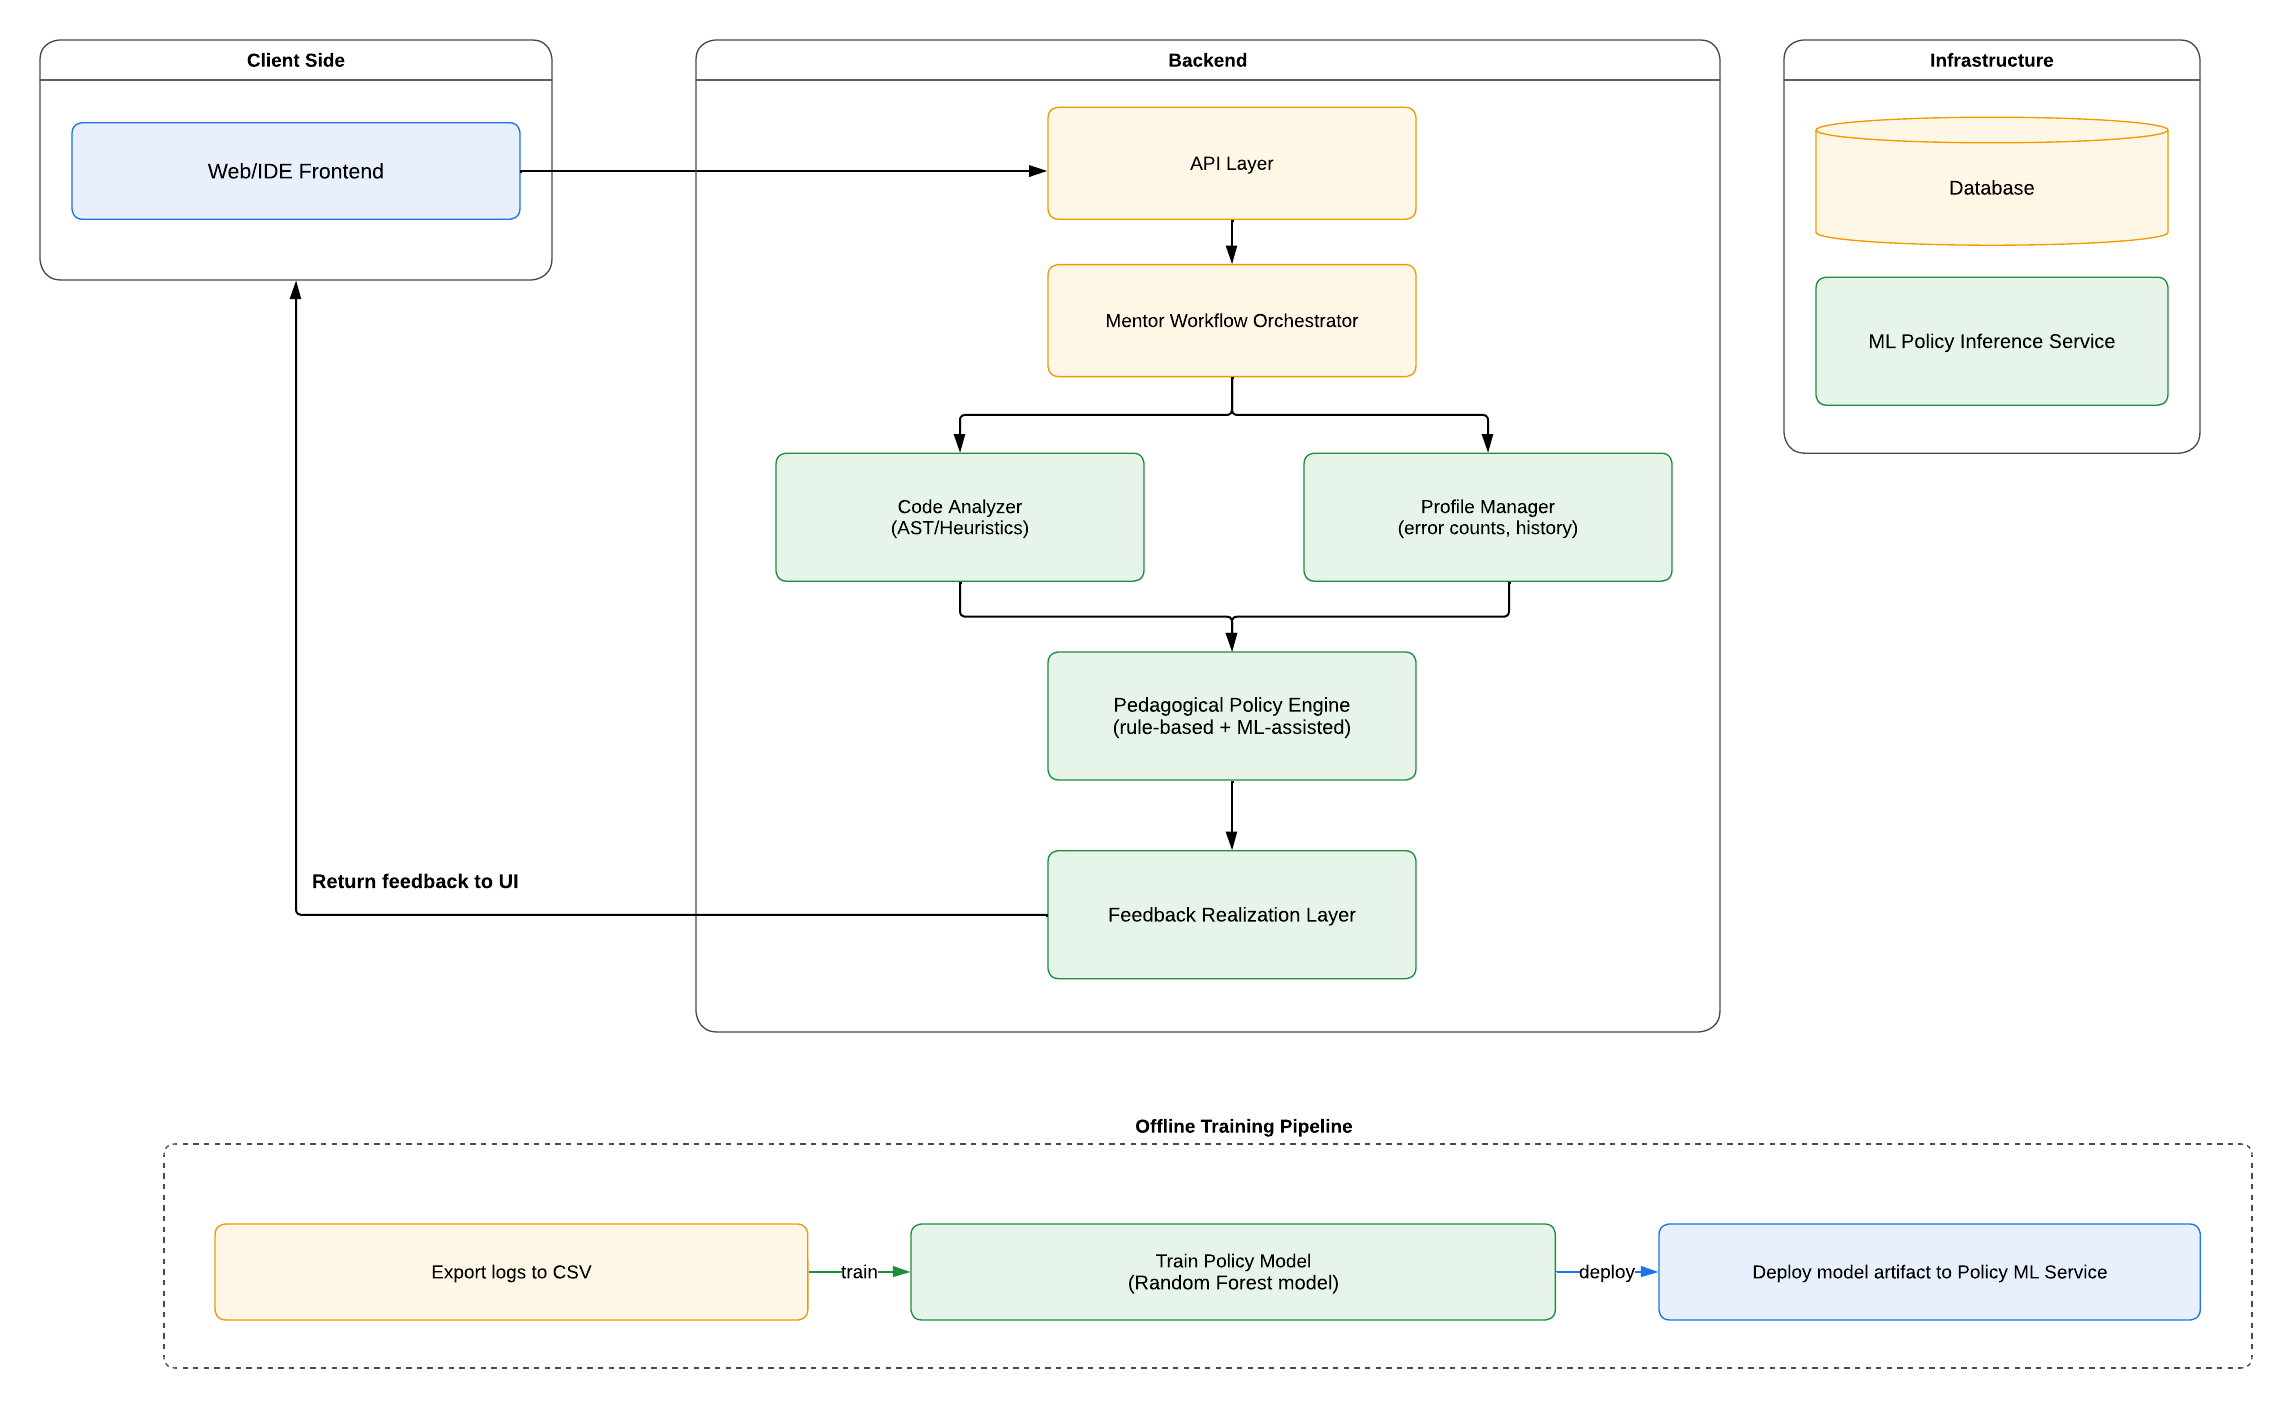
\includegraphics[width=\linewidth]{arch-SIST.png}
\caption{SocratesAI architecture: analyzer signals and session state are processed before feedback realization. The LLM is used after action selection, not as the core policy.}
\label{fig:architecture}
\end{figure}

\subsection{Analyzer and Session State}

The analyzer converts a code snapshot into a compact event descriptor. In the current prototype, this descriptor includes compile success, tests passed and failed, error type, severity, code length, and suspicious region. The analyzer is deliberately lightweight. It is not expected to understand every possible student program; its role is to provide structured signals for the mentoring decision.

The session state records signals that are useful during one problem-solving session: repeated error type, total errors seen, attempt number, previous feedback action, previous feedback success, and total feedback count. This is not a full knowledge-tracing model. It is closer to what a teaching assistant may keep in mind during a short lab conversation: whether the student has already seen the same problem and whether direct help was recently given.

\subsection{Policy Layer}

The policy selects one of four actions:

\begin{itemize}
    \item \texttt{CODE\_HIGHLIGHT}: point to a suspicious region with little explanation;
    \item \texttt{CONCEPTUAL\_HINT}: give a short reminder about the concept;
    \item \texttt{GUIDING\_QUESTION}: ask a question that makes the student inspect their own code;
    \item \texttt{NO\_FEEDBACK}: stay silent when intervention is not useful or evidence is weak.
\end{itemize}

Formally, the analyzer maps the code state $c_t$ into an event descriptor $e_t$. The profile manager maintains session state $s_t$, and the policy chooses action $a_t$:

\[
\pi(e_t, s_t) \rightarrow a_t,\quad a_t \in \{\texttt{HL}, \texttt{CH}, \texttt{GQ}, \texttt{NF}\}.
\]

The current implementation supports a rule policy and an ML policy. The ML policy is a multi-class Random Forest classifier served through a FastAPI inference service. It uses the same runtime features as the rule policy: error type, severity, compile result, test outcomes, recurrence counts, attempt number, previous action, previous action success, suspicious-region flag, code length, and feedback count.

\subsection{Feedback Realization}

Feedback realization is separate from policy selection. In the deterministic path, templates produce the message. In the LLM path, Gemini 2.5 Flash-Lite receives the selected pedagogical action and analyzer metadata, with instructions to avoid full solutions and corrected code. If Gemini is disabled or fails, the system falls back to templates. In the latest benchmark, the response source was recorded so that LLM responses and template fallbacks could be separated.

\section{Methodology}

The evaluation is a prototype-based system study. It measures runtime behavior, action-selection quality, and model-development evidence. It does not claim statistically validated learning gains.

\begin{table*}[t]
\centering
\caption{Evaluation Artifacts}
\label{tab:artifacts}
\renewcommand{\arraystretch}{1.15}
\begin{tabular}{p{3.3cm} p{2.3cm} p{9.0cm}}
\toprule
\textbf{Artifact} & \textbf{Size} & \textbf{Purpose} \\
\midrule
Real-HTTP replay & 570 events & Measures backend mentoring-loop responsiveness with PostgreSQL and template feedback. \\
Concurrent smoke test & 400 requests & Checks stability under eight-way parallel load. \\
Fixed ML+Gemini problem suite & 360 events & Primary end-to-end benchmark for action agreement and LLM feedback realization. \\
Rubric policy dataset & 1,080 rows & Supervised action-selection dataset with \texttt{target\_feedback\_action}. \\
Expanded weak-label dataset & 381,003 rows & Large-scale classifier comparison and feature ablation. \\
\bottomrule
\end{tabular}
\end{table*}

The 12-problem suite includes palindrome checking, two-sum, valid parentheses, binary search, merge sorted array, trapping rain water, LRU cache, longest substring without repeating characters, reverse linked list, matrix diagonal sum, Roman-to-integer conversion, and climbing stairs. Each problem is replayed as a six-step sequence: syntax issue, unfinished implementation, first conceptual mistake, repeated conceptual mistake, partial compiling logic, and local completion. The target action is defined by a review rubric for each event.

The latest benchmark used Docker Compose, PostgreSQL, the Spring Boot backend, the FastAPI ML policy service, and Gemini 2.5 Flash-Lite. Fresh synthetic student identifiers were used to avoid contamination from previous session history. The main metrics are action agreement, macro F1, per-class precision/recall/F1, per-problem agreement, runtime errors, latency, and feedback source.

For model development, the study compared a rule baseline, logistic regression, random forest, XGBoost, LightGBM, and a small neural classifier. Ablations removed history features, analyzer features, suspicious-region information, and previous-feedback-action information. This was done to check whether the architecture carries measurable signal beyond the LLM realization step.

\section{Results}

\subsection{Backend Responsiveness}

In the 570-event real-HTTP replay, all requests completed successfully. Mean request latency was 44.11 ms, median latency was 46 ms, P95 latency was 58 ms, and P99 latency was 68 ms. The analyzer time averaged 6.81 ms with P95 of 10 ms. Under an additional 400-request stress smoke test at concurrency level 8, all requests completed successfully with mean latency of 37.59 ms, P95 latency of 56 ms, and P99 latency of 61 ms.

\subsection{ML+Gemini Action Quality}

The primary current benchmark is the fixed ML+Gemini problem-suite run. The system processed 360 events across 12 problems and five fresh cohorts. All requests completed successfully. The policy matched the target rubric action in 95.83\% of events and reached 95.80\% macro F1. Mean wall latency was 1079.21 ms and P95 latency was 2072 ms. Gemini produced 317 feedback messages, while 43 responses used deterministic template fallback.

\begin{table}[t]
\centering
\caption{Fixed ML+Gemini Problem-Suite Benchmark}
\label{tab:mlgemini}
\renewcommand{\arraystretch}{1.12}
\begin{tabular}{lc}
\toprule
\textbf{Metric} & \textbf{Value} \\
\midrule
Events & 360 \\
Successful requests & 360 \\
Runtime errors & 0 \\
Action agreement & 95.83\% \\
Macro F1 & 95.80\% \\
Mean latency & 1079.21 ms \\
P95 latency & 2072 ms \\
Gemini responses & 317 \\
Template fallbacks & 43 \\
\bottomrule
\end{tabular}
\end{table}

\begin{figure}[t]
\centering
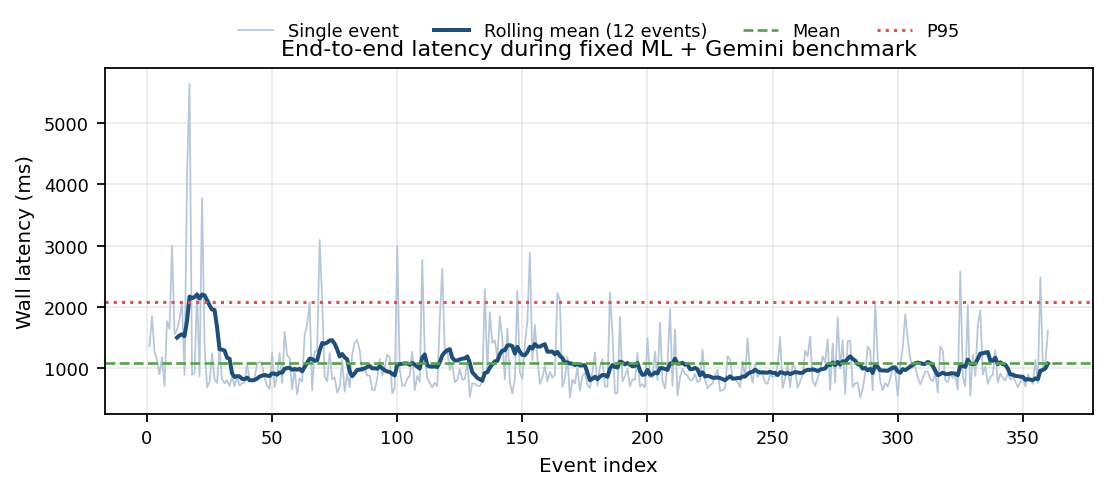
\includegraphics[width=\linewidth]{sist_latency_timeline.png}
\caption{End-to-end latency during the fixed ML+Gemini benchmark.}
\label{fig:latency}
\end{figure}

Table~\ref{tab:classmetrics} reports per-class metrics. The strongest class was \texttt{GUIDING\_QUESTION}, where the policy reached 100\% precision and recall. \texttt{NO\_FEEDBACK} remained the weakest class because several local-completion states still triggered an intervention.

\begin{table}[t]
\centering
\caption{Per-Class Action Metrics}
\label{tab:classmetrics}
\small
\renewcommand{\arraystretch}{1.12}
\begin{tabular}{lcccc}
\toprule
\textbf{Action} & \textbf{P} & \textbf{R} & \textbf{F1} & \textbf{N} \\
\midrule
\texttt{CODE\_HIGHLIGHT} & 95.24 & 100.00 & 97.56 & 100 \\
\texttt{CONCEPTUAL\_HINT} & 93.10 & 96.43 & 94.74 & 140 \\
\texttt{GUIDING\_QUESTION} & 100.00 & 100.00 & 100.00 & 60 \\
\texttt{NO\_FEEDBACK} & 100.00 & 83.33 & 90.91 & 60 \\
\bottomrule
\end{tabular}
\end{table}

\begin{figure}[t]
\centering
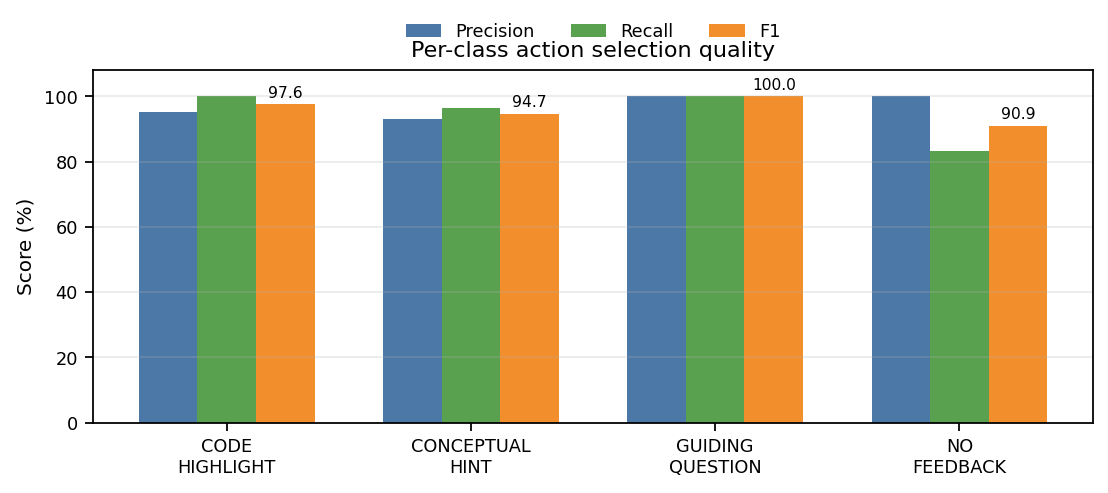
\includegraphics[width=\linewidth]{sist_per_class_metrics.png}
\caption{Per-class precision, recall, and F1 for feedback-action selection.}
\label{fig:classbars}
\end{figure}

Problem-level agreement is shown in Fig.~\ref{fig:problemagreement}. Ten out of twelve tasks reached 100\% agreement. The weaker cases were \texttt{lru-cache} and \texttt{valid-parentheses}. The 15 disagreements were concentrated in local-completion and unknown-logic states, which gives a clear target for the next analyzer improvement.

\begin{figure}[t]
\centering
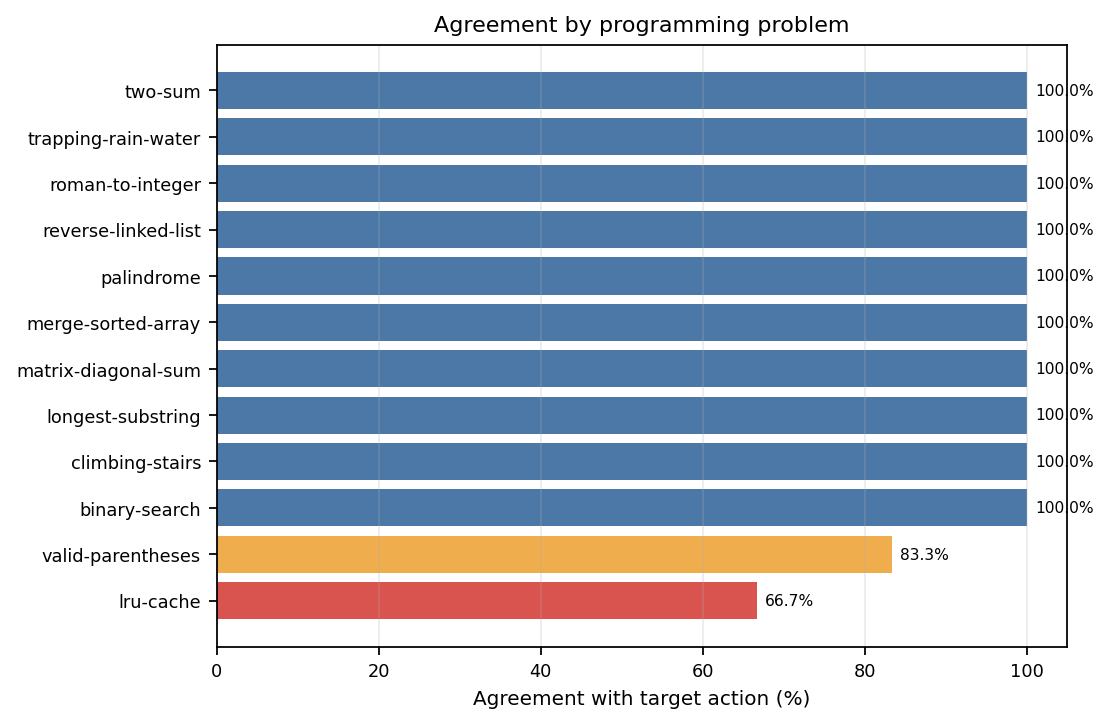
\includegraphics[width=\linewidth]{sist_problem_agreement.png}
\caption{Agreement with target feedback action by programming problem.}
\label{fig:problemagreement}
\end{figure}

\subsection{Model Comparison and Ablation}

The expanded weak-label dataset contains 381,003 rows derived from 117,232 coding sessions. The final Random Forest training run used a problem-level group holdout with 303,515 training rows and 77,488 test rows. It reached 1.0000 accuracy and 1.0000 macro F1 when trained to reproduce the current policy labels. This score is expected because the labels are weak proxy labels from the policy behavior; it should be interpreted as a pipeline and scale check.

The 1,080-row rubric problem-suite dataset was also evaluated with group holdout by problem. The classifier trained on 810 rows and tested on 270 rows from held-out problems. It reached 1.0000 action accuracy and 1.0000 macro F1, showing that the rubric labels are learnable from the runtime feature set.

The more useful model-development result is the ablation. When analyzer features were removed from the expanded dataset, model performance dropped to 92.32\% accuracy and 88.13\% macro F1. This supports the design decision to keep structured code-analysis features in the policy layer instead of relying only on generic feedback generation.

\begin{figure}[t]
\centering
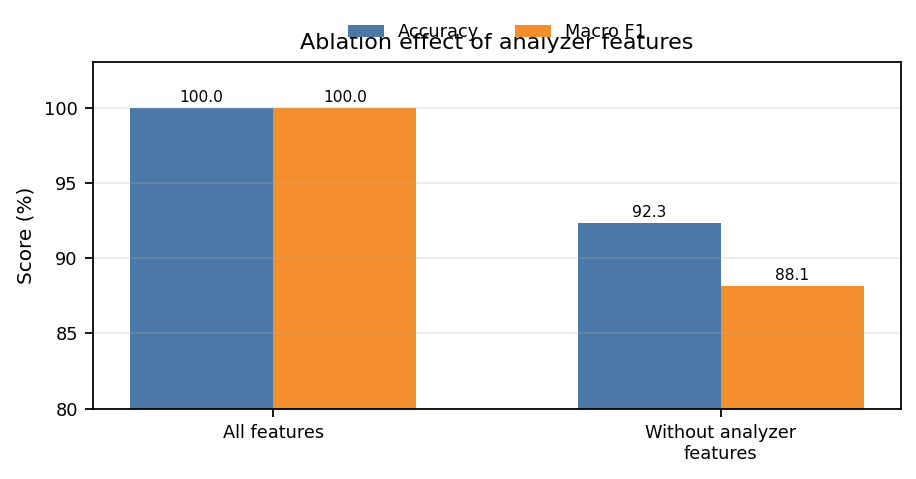
\includegraphics[width=.88\linewidth]{sist_ablation_analyzer_features.png}
\caption{Ablation effect of analyzer features on the expanded weak-label dataset.}
\label{fig:ablation}
\end{figure}

\subsection{Baseline Context}

A fixed no-policy selector that always returns a conceptual hint reached only 38.89\% action agreement and 14.00\% macro F1 in the deterministic 12-problem baseline run. This baseline is simple, but useful. It shows that generic feedback cannot replace action selection: it cannot highlight a region, ask a question, or stay silent when the best action is no feedback.

\section{Discussion}

The main result is not that an LLM can produce a short message. That is already known. The more important result is that the system can choose a bounded feedback action before message generation and preserve this action structure in a real runtime loop. This makes the mentor more inspectable for instructors and safer for CS1 students than an unrestricted chat assistant.

The results also answer the main criticism from the earlier rejected version of this work. The experimental scale is now clearer: the paper reports event counts, task coverage, dataset sizes, model splits, and benchmark conditions. The technical depth is stronger because the work now includes model families and ablations, not only latency numbers. The novelty is also more explicit: SocratesAI is not presented as another LLM helper, but as a policy-controlled mentoring pipeline where the LLM is a realization component.

At the same time, the evidence boundary remains important. These results are system-level and action-level evidence. They do not prove that students learn more, retain concepts longer, or become better debuggers. To make that stronger claim, the next study needs student-level pre-tests, post-tests, delayed tasks, and comparison conditions.

\section{Limitations and Future Work}

The first limitation is that the benchmark is still controlled and event-level. It covers 12 tasks and repeated coding states, but it is not a real classroom deployment. The second limitation is that the 381,003-row dataset is weakly labelled. It is useful for scale and ablation, but it is not the same as instructor-labelled classroom feedback. The third limitation is the remaining weakness in \texttt{NO\_FEEDBACK}. Local-completion cases in \texttt{lru-cache} and \texttt{valid-parentheses} still sometimes receive an intervention.

The next step is to collect 200--500 manually reviewed events from real use. A second rater should label an overlapping subset of 50--100 events so that Cohen's kappa can be reported. The system should also log outcome labels such as whether the student fixed the error after feedback, how long the fix took, and whether the same error appeared again. These labels are necessary before making a stronger educational claim.

\section{Conclusion}

This paper presented SocratesAI, a policy-guided real-time mentor for introductory programming. The system separates analyzer signals, session state, feedback-action selection, and feedback realization. This separation makes the feedback strategy explicit and allows an LLM to be used in a bounded role rather than as an unconstrained tutor.

The evaluation showed that the backend mentoring loop can operate with low latency, that the fixed ML+Gemini runtime pipeline can match target feedback actions with 95.83\% agreement and 95.80\% macro F1 on a 12-problem benchmark, and that analyzer-derived features are important for policy prediction. These findings support the technical feasibility of policy-guided mentoring for CS1. The next research step is a classroom study that connects event-level behavior with student-level learning outcomes.

\nocite{Francisco2022}
\nocite{Chrysafiadi2022}
\nocite{pankiewicz2023largelanguagemodelsgpt}
\nocite{AutomatedAssessmentToolsForGrading2022}
\nocite{FeedbackSystemSupportingStudents2022}
\nocite{EvaluationofLLMtoolsforfeedbackgeneration}
\nocite{AutomatingHumanTutorStyleProgrammingFeedback}
\nocite{AITutoringinSDEducation}
\bibliographystyle{IEEEtran}
\bibliography{references}

\end{document}
